\chapter{Problem Analysis}
Throughput prediction for wireless networks is inherently difficult. This paper explores the use of a multistage approach to throughput prediction using deep learning based techniques. There are numerous considerations before trying to model any time series problem such as availability of relevant data, selection of model, feature selection, imputation etc. There are also more application specific items to consider such as how long of a history window should be used for predictions or how far into the future should be predicted? How to decompose the problem also influences the architecture of a multistage approach. This section explores these issues.

\section{Understanding the Dataset}
The dataset used in this paper was collected by researchers in University College Cork in and around the greater Cork City area. Data was collected using an Android network monitoring application, G-NetTrack Pro. Apple devices currently do not have any equivalent application for collecting cellular network analytics. The dataset is a collection of 135 different traces approximately 15 minutes in length on average. Traces were collected by the UCC researchers under a number of different movement patterns. The traces are divided based on the following movement patterns:

•\textbf{Static}: The trace was collected while the mobile devices location remained fixed. This is characteristic of a common use case for mobile devices such as watching video while seated at a desk. Such a use case presents the best case scenario for a cellular network as the connection will experience low variability in its stability.

•\textbf{Car}: The trace was collected while travelling in Cork city and its surrounding suburbs by car.

•\textbf{Train}: The trace was collected while travelling by train. These traces contain a mix of both 4G and 3G as availability for 4G networks was in urban areas only at the time these experiments took place.

•\textbf{Bus}: Traces collected while using public transport around Cork City.

•\textbf{Pedestrian}: Traces collected while walking around Cork City center using different routes.

Traces were collected at a variety of times on both weekdays and weekends in order to provide adequate depiction of congestion patterns. The dataset includes of a number of physical layer metrics, as well has GPS metrics and the upload and download bitrate. The following description of the metrics collected was taken directly from the paper \cite{inproceedings} written by the researchers involved in the construction of this dataset. For a more in depth understanding of the dataset I recommend reading their paper. All credit goes to them for the following description of the metrics:

•Timestamp: timestamp of sample \\
•Longitude and Latitude: GPS coordinates of mobile device \\
•Velocity: velocity in kph of mobile device \\ 
•Operatorname: cellular operator name (anonymised) \\
•CellId: Serving cell for mobile device \\
•NetworkMode: mobile communication standard (2G/3G/4G) \\
•RSRQ: value for RSRQ. RSRQ Represents a ratio between RSRP and Received Signal Strength Indicator (RSSI). Signal strength (signal quality) is measured across all resource elements (RE), including interference from all sources (dB). \\
•RSRP: value for RSRP. RSRP Represents an average power over cell-specific reference symbols carried inside distinct RE. RSRP is used for measuring cell signal strength/coverage and therefore cell selection (dBm). \\
•RSSI: value for RSSI. RSSI represents a received power (wide-band) including a serving cell and interference and noise from other sources. RSRQ, RSRP and RSSI are used for measuring cell strength/coverage and therefore cell selection(handover) (dBm)0\\
•SNR: value for signal-to-noise ratio (dB). \\
•CQI: value for CQI of a mobile device. CQI is a feedback provided by UE to eNodeB. It indicates data rate that could be transmitted over a channel (highest MCS with a BLER probability less than 10\%), as the function of SINR and UE’s receiver characteristics. Based on UE’s prediction of the channel, eNodeB selects an appropriate modulation scheme and coding rate. \\
•DL\_bitrate: download rate measured at the device (application layer) (kbit/s) \\
•UL\_bitrate: uplink rate measured at the device (application layer) (kbit/s) \\
•State: state of the download process. It has two values, either I (idle, not downloading) or D (downloading) \\
•NRxRSRQ \& NRxRSRP: RSRQ and RSRP values for the neighbouring cell. \\
•Cell\_Longitude \& Cell\_Latitude: GPS coordinates of serving eNodeB. We use OpenCelliD4, the largest community open database providing GPS coordinates of cell towers. \\
•Distance: distance between the serving cell and mobile device in metres.

\newpage
\section{Considerations of the Dataset}

As the dataset is a collection of separate traces (experiments), this must be taken into account when constructing train and test splits. The entire dataset cannot be viewed a a series of disconnected time series as traces start from different physical locations, run for different lengths of time and use the same workload as a starting point for measuring network data. As such special care must be taken in order to ensure proper construction of train-test sequences.

The dataset contains considerable missing values for some network features such as NRxRSRP \& NRxRSRQ. Lstm based machine learning techniques require complete data. As such imputation had to be carried out to fill in these gaps. There are various methods of imputation such as mean imputation, max or min imputation, K nearest neighbours (knn) based imputation methods and more. Some of these methods were considered in this project but it is important to note that no imputation method is perfect. Understanding of the missingness observed in the data may lead to choosing one method over the other. 

Methods like knn imputation also require considerable computational power \& space in memory compared to other more simple methods. This limits the usefulness of such a method to the training phase of a throughput predictor only. Knn or other complex imputation methods would not be viable for deployment directly on the mobile device due to the space and computational constraints of mobile devices. Edge computing would allow for more complicated imputation methods however there is also a time penalty for more complicated methods.

Some features collected are not reported directly by the G-NetTrack Pro such as cell tower location data. As such these features were excluded from consideration in this project. If such information was made more readily available in the future it may prove useful in throughput prediction applications however this is outside the scope of the project.

While this dataset is robust in its construction and depiction of typical mobile communication system scenarios, it is not universal. Mobile network infrastructure implementations vary heavily by location. This dataset contains a mix of 2G/3G/4G networks. Older wireless communication technologies have different network environment distributions. As technology continues to progress the model will suffer from distribution shift.

\section{Choice of History \& Horizon Windows}
A typical input for an Lstm model used in forecasting takes the shape of: $[ n, p, q ]$ where n is the number of examples, p is the length of the history window and q is the number of features. The output will then be in the form of $[n, k, s ]$ where k is the length of the horizon window and s is the number of target variables the model predicts, typically s=1. Fig \ref{fig:example_of_ts} illustrates the construction of a single example in the univariate case.

\begin{figure}[h]
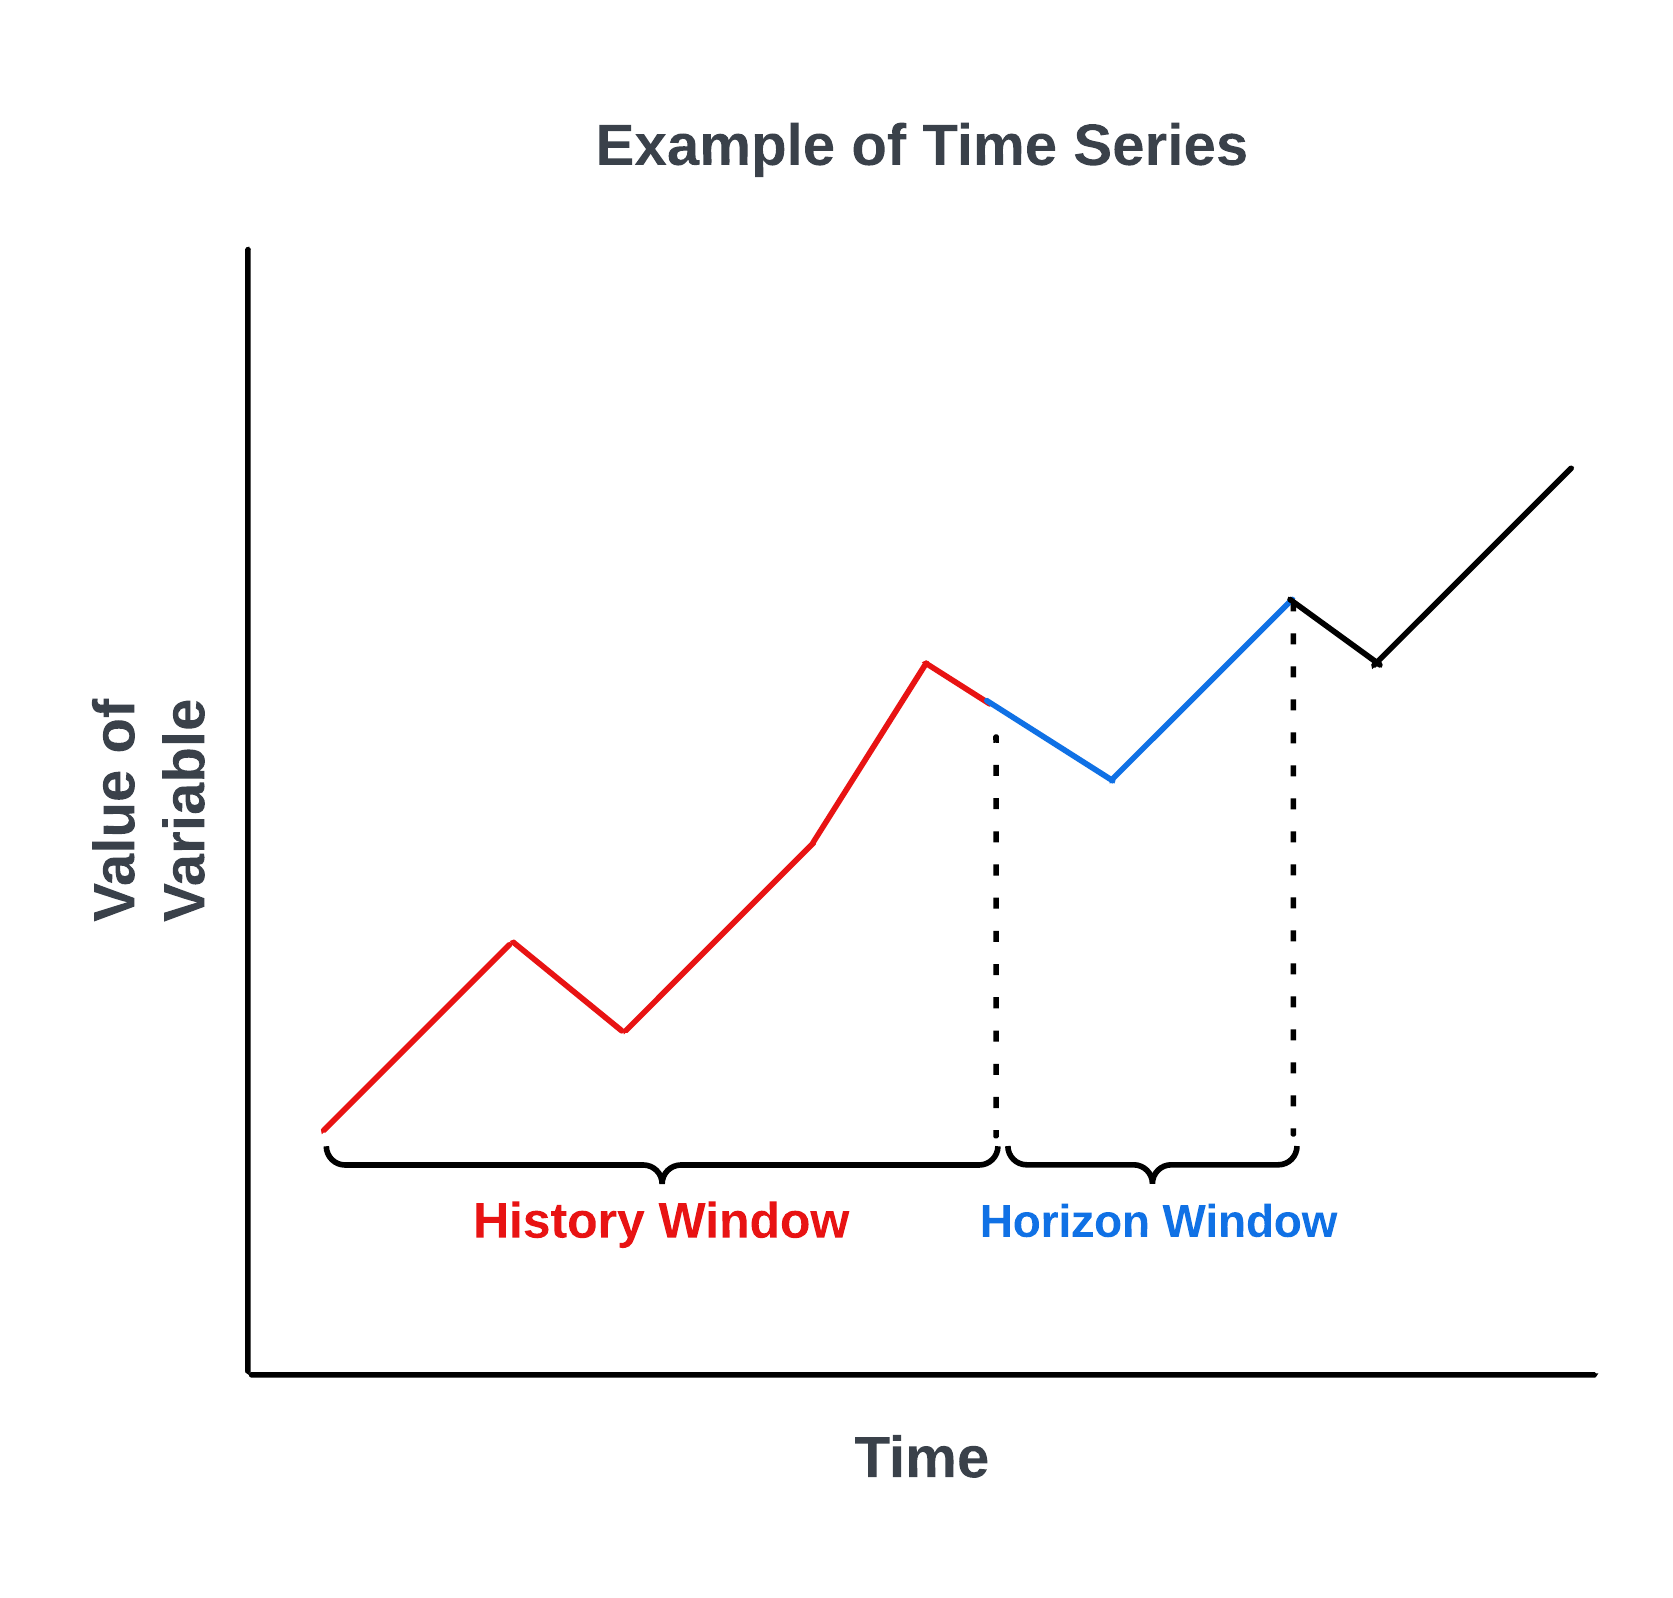
\includegraphics[scale=0.15]{History Horizon.png}
\caption{Graph showing how a history and horizon window can be constructed for a feature in time series data}
\label{fig:example_of_ts}
\end{figure}

In general a larger history window leads to a better prediction \cite{}. There are many methods for identifying the optimal length of the horizon and history windows. The application the model is being deployed in will also place restrictions on 


\section{Identifying Bounds for Mutlistage Models}
Two multistage approaches for modelling throughput prediction were considered in this paper. Each of the two architectures however share the same base models. The first model is a simple classifier that aims to predict a future throughput as one of 3 distinct situations, low throughput, medium throughput or high throughput. The choice to divide the problem based on the value of the download throughput comes from the fact that traces typically reported throughput above certain bounds (5Mbps, 1Mbps etc) far more often than below them. This imbalance leads to a single stage model frequently overestimating in low/medium throughput situations. Overestimating in these low or medium throughput scenarios leads to a noticeable decrease in the perceived quality of delivery in applications such as video streaming. 

The choice of the number of bounds (and subsequently models) and how to classify a given sequence of input data is arbitrary. For the purposes of this paper, dividing the data into one of three bounds sufficed. The following download throughput ranges were chosen to label given sequences of data:

•Low: $ y< 1Mbps$ \\
•Medium: $1Mpbs \leq y \leq 5Mpbs$ \\
•High: $y > 5Mbps$ \\

For forecasting, Lstm models are typically trained on x, y pairs where x is historic data of the predictor features over the past p seconds and y is the true value of the target variable of the next k seconds. As seen above, y is used to classify a given pair as an example of either low, medium or high throughput.